\chapter{analyse et conception}

Pour ce problème, les méthodes exactes ne sont pas suffisamment performantes pour résoudre de grandes instances dans des délais raisonnables.
La qualité d'une méthode exacte est estimée à partir de plusieurs critères :
\begin{itemize}
	\item Le temps de calcul nécessaire pour trouver la solution en fonction de la taille de l'instance.
	\item L'espace mémoire requit pour résoudre l'instance en fonction de la taille de l'instance.
	\item L'efficacité de la parallélisation de la méthode.
\end{itemize}
Pour des résultats plus rapides, il faut passer par des méthodes heuristiques.
Ces méthodes permettent de trouver plus rapidement une solution correcte, mais pas forcément la meilleure.
Pour évaluer une méthode heuristique, il faut prendre en compte les critères suivants :
\begin{itemize}
	\item La qualité de la solution en fonction du temps et de la taille de l'instance.
	\item L'espace mémoire utilisé en fonction de la taille de l'instance.
	\item L'écart de qualité de la solution par rapport a celle de la méthode exacte en fonction du temps.
	\item Le temps qu'il faut pour obtenir une solution correcte par rapport a la méthode exacte.
\end{itemize}
Pour évaluer une méthode heuristique, il faut une méthode exacte pour faire la comparaison.

\section{méthode exacte}
\label{section:analyse:methode_exacte}
Hugo Chevroton a proposé une méthode pour résoudre le sous-problème pour lequel les ordres des jobs et les lots sont fixés,
cette méthode utilise un solveur et est présentée dans la partie \autoref{appendix:modelisation_initiale}.

Je me base sur sa modélisation pour ajouter la liberté sur les ordres des jobs dans les lots.

\section{Paramètres}
\begin{labeling}{paramètres}
	\item [$m$]
	Nombre de machines
	\item [$n$]
	Nombre de jobs.
	\item [$V$]
	Nombre de lots.
	\item [$N_k$]
	Nombre de job du lot $k$.
	\item [$p_{i, j}$]
	Durée de travail sur la machine $i$ pour le job $j$.
	\item [$h_{j}^{WIP}$] 
	Cout d'inventaire pendant la production du job $j$.
	\item [$h_{j}^{FIN}$] 
	Cout d'inventaire après la production du job $j$.
	\item [$a_k$]
	Date de départ au plus tôt du lot $k$.
	\item [$b_k$]
	Date de départ du lot k a partir de laquelle les couts d'inventaires sont minimisé.
	\item [$\lambda_k$]
	Nombre de segment de la fonction $F_k$
	\item [$\alpha_{k, s}$]
	Cout de chaque unité de temps dans le segment $s$ de la fonction $F_k$.
	\item [$c_{k, s}$]
	Cout des pénalités de retard pour le $s$\ieme segment de la fonction $F_k$.
	\item [$t_{k, s}$]
	Date de début du $s$\ieme segment de la fonction $F_k$, $t_{k, \lambda_k+1}$ vaut $b_k$.
	
\end{labeling}


\section{Variables}

\begin{labeling}{variables}
	\item [$x_{k, s}$]
	Vaut 0 ou 1 si la date de départ du lot $k$ est dans le segment $s$ de la fonction $F_k$.
	\item [$d_{k, s}$]
	Représente le temps écoulé dans le segment $s$ avant le départ du lot $k$.
	\item [$C_{i, j}$]
	Date de fin du travail de la machine $i$ sur le job $j$.
	
	\item [$y_{j1,j2}$]
	Variable de précédences en production, vaut 1 si le job $j1$ est effectué avant le job $j2$.
	\item [$j_k$]
	Dernier job du lot $k$.
	\item [$F_k$] 
	Date de fin de production du lot $k$.
	
	\item [$IC^{WIP}$]
	Cout d'inventaire pendant la production.
	$$IC^{WIP}= \sum_{j=1}^{n} \sum_{i=1}^{m-1} \left(C_{i+1, j} - p_{i+1, j} - C_{i, j} \right) h_j^{WIP}$$
	\item [$IC^{FIN}$]
	Cout d'inventaire entre la fin de la production et la livraison des jobs.
	$$IC^{FIN} = \sum_{k=1}^{V} \sum _{j\in j^k} \left( F_k - C_{m, j} \right) h_j^{FIN}$$
	\item [$IC$]
	Couts d'inventaire total.
	$$IC = IC^{WIP} + IC^{FIN}$$
\end{labeling}


\section{Objectif}
Somme des coûts à minimiser
$$IC + \sum_{k=1}^{V} \sum_{s=1}^{\lambda_k} \left(x_{k, s} c_{k, s}+ d_{k,s} \alpha_{k, s} \right)$$

\section{Contraintes}

\begin{itemize}
	\item
	      Lien entre la fin du dernier job d'un lot et le départ du lot
	      \begin{align}
		      C_{j_k, m} \leq \sum_{s=1}^{\lambda_k} \left( x_{k,s} t_{k, s} + d_{k, s} \right) &  & \forall k \in \left\{i, \cdots, V \right\}
	      \end{align}
	\item
	      La date de départ en livraison ne peut faire partie que d'un segment de la fonction $F_k$.
	      \begin{align}
		      \sum_{s=1}^{\lambda_k} x_{k, s} = 1 &  & \forall k \in \left\{i, \cdots, V \right\}
	      \end{align}
	\item
	      Chaque segment n'est utilisé que si il contient la date de départ du lot.
	      \begin{align}
		      d_{k, s} \leq x_{k, s} \left( t_{k, s+1 - t_{k, s} -1} \right) &  & \forall k \in \left\{i, \cdots, V \right\}, \forall s \in \left\{1, \cdots, \lambda_k\right\} \\
		      0 \leq d_{k, \lambda_k}                                        &  & \forall k \in \left\{i, \cdots, V \right\}
		  \end{align}
	% 
	\item
	      Chaque job est soit le successeur soit le prédécesseur de chacun des autres jobs.
	      \begin{align}
		      y_{j1,j2}+y_{j2,j1}=1 &  &
		      \forall j1,j2\in\left\{1,\dotsc,n\right\}, j1<j2
	      \end{align}
	\item
	      Les jobs ne peuvent pas être leurs propres successeurs.
	      \begin{align}
		      y_{j,j}=0 &  &
		      \forall j\in \left\{1,\cdots, n\right\}
	      \end{align}
	\item
	      Contrainte de gamme, les machines ne peuvent pas travailler sur plusieurs jobs simultanément.
	      Cette contrainte assure également que les jobs sont produits dans l'ordre prescrit.
	      \begin{align}
		      C_{i,j2} \geq C_{i,j1}+p_{i,j2}-M y_{j1,j2} &  &
		      \forall i\in\left\{1,\dotsc,m\right\}, \forall\left(j1,j2\right)\in\left\{1,\cdots,n\right\}^2
	      \end{align}
	\item
	      Contrainte de précédence, une machine ne peut pas travailler sur un job tant que la machine précédente n’a pas terminé de travailler dessus.
	      Cette contrainte assure également que les tâches des jobs sont produit dans l'ordre prescrit.
	      \begin{align}
		      C_{i,j}\geq C_{i-1,j}+p_{i,j} &  &
		      \forall j\in\left\{1,\cdots,n\right\},\forall i\in\left\{2,\dotsc,m\right\}
		  \end{align}
	\item 
		Un job est terminé quand toutes ces tâches sont terminées.
		\begin{align}
			f_j \geq C_{m, j} & & \forall j \in \left\{0,\dotsc,n\right\}
		\end{align}
	\item
	      Un lot ne peut être livré que si tous ces jobs sont terminés.
	      \begin{align}
		      F_k \geq C_{m, j} &  & \forall k \in \left\{1,\dotsc, n \right\}, \forall j \in J^k
	      \end{align}
\end{itemize}

Les contraintes suivantes servent à accélérer la résolution du problème.
\begin{itemize}
	\item
	      La date de fin du lot $k$ optimal est entre les dates $a_k$ et $b_k$ calculé au préalable.
	      \begin{align}
		      a_k \leq C_{j_k, m} \leq b_k &  & \forall k \in \left\{1,\cdots,V\right\}
	      \end{align}
	\item
	      Le temps écouler dans un segment de $F_k$ avant le départ d'un lot ne doit pas faire partir le lot après $b_k$.
	      \begin{align}
		      d_{k, \Lambda_k} \leq t_{k s+1} - t_{k, s} &  & s \in \left\{1,\cdots,\lambda_k\right\}, \forall k \in \left\{1,\cdots,V\right\}
	      \end{align}
	\item
	      La date du départ d'un lot ne peut pas précéder le début du segment auquel il appartient.
	      \begin{align}
		      x_{k, s^t} t_{k, s} \leq C_{j_k, m} &  & s \in \left\{1,\cdots,\lambda_k\right\}, \forall k \in \left\{1,\cdots,V\right\}
	      \end{align}
\end{itemize}


\section{méthode heuristique}
\label{section:analyse:methode_heuristique}

Pour la méthode heuristique, j'ai décidé avec mon encadrant d'utiliser un algorithme de recherche locale.
Cet algorithme est présenté dans la partie \autoref{section:recherche_locale}.
	
Les solutions sont représentées par une liste de jobs classés dans l'ordre de leurs réalisation.

\subsection{Operateur de voisinage}

L'opérateur à pour rôle de définir les solutions voisines de la solution principale.

Pour ce projet, deux opérateurs ont été envisagés :

\begin{itemize}
	\item Un opérateur qui donne des solutions où les emplacements de deux jobs dans l'ordre de production ont été échangé.
	\item Un opérateur qui donne des solutions où l'emplacement d'un job dans l'ordre de réalisation a été changé.
	Cet opérateur permet de conserver des séquences de jobs qui peuvent être bon.
\end{itemize}

\subsection{Exploration du voisinage}

Il existe plusieurs façons d'explorer le voisinage fourni par un opérateur, dans ce projet, deux stratégies ont été testé :
\begin{itemize}
	\item Meilleur amélioration :
	
	Cette stratégie consiste à évaluer tout les voisins de la solution actuelle et de prendre le meilleur.
	Le défaut avec cette méthode est qu'il y a un grand nombre de solutions évalué, ce qui fait que chaque itération de la recherche prend du temps.
	\item Première amélioration : 
	
	Cette stratégie consiste à sélectionner le premier voisin qui est meilleur que la solution actuel.
	Cette stratégie permet de ne pas évaluer tout les voisins et d'itérer plus rapidement, ce qui permet d'explorer plus de minimum locaux dans le temps impartie.
\end{itemize}

\subsection{Stratégie de sortie des minimum locaux}
Lorsque la solution étudiée n'a pas de meilleur voisin, on est dans un minimum local.
Il existe plusieurs façon de sortir des minimum locaux, dans ce projet, on à choisi de relancer une recherche locale à partir d'une nouvelle solution aléatoire.


\subsection{Condition d'arrêt}
Une fois dans un minimum local, l'algorithme repart sur une solution aléatoire, il n'y à donc pas de fin.
Pour arrêter la recherche, il faut une définir une condition arrêt.
Pour ce projet, on a choisi de limiter le temps accordé à la recherche local.

Lorsque la recherche locale atteint un minimum local, si le temps n'est pas écoulé, la stratégie de sortie des minimums locaux est utilisé.
Lorsque le temps est écoulé, la recherche local termine la recherche du minimum local en cours.

Cette durée minimum pour la recherche local est définit à l'exécution par l'utilisateur de l'application.

\section{Modélisation logicielle}

D'un point de vu logiciel, le projet est séparé en plusieurs parties, 
chaque méthode de résolution est implémentée dans un projet Visual Studio distinct et
le code en commun est placé dans une bibliothèque.

\subsection{Bibliothèque}

La bibliothèque définit les structures de données des instances et solutions.
Elle contient également des classes pour lire les instances, valider les solutions et écrire les solutions.

\subsubsection{Structures de données}

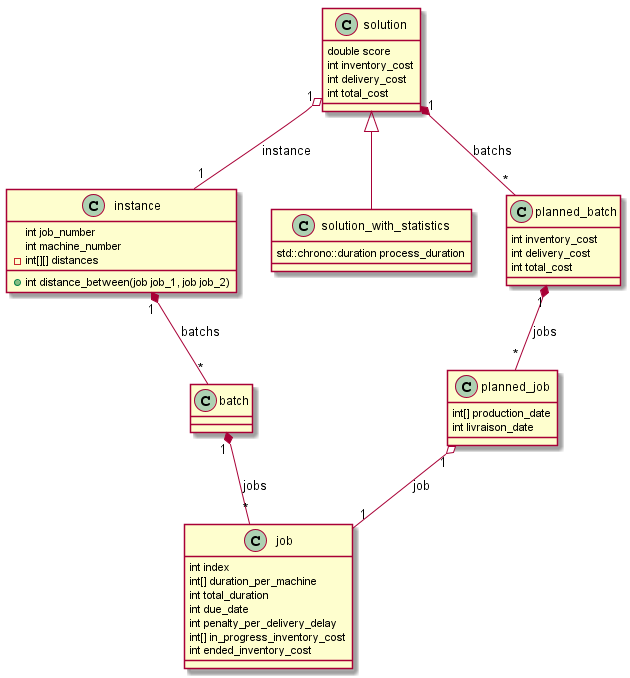
\includegraphics[width=\textwidth]{parts/analyse_et_conception/diagramme_data}

Les classes \detokenize{planned_batch} et \detokenize{planned_job} représentent les lots et jobs qui ont été planifiés.
La durée de la résolution ne fait pas partie de la solution,  cette donnée ne concerne que la méthode qui génère la solution.

La classe \detokenize{solution_with_statistiques} étend la classe solution, 
elle ajoute la durée de la résolution.

\subsubsection{Services}

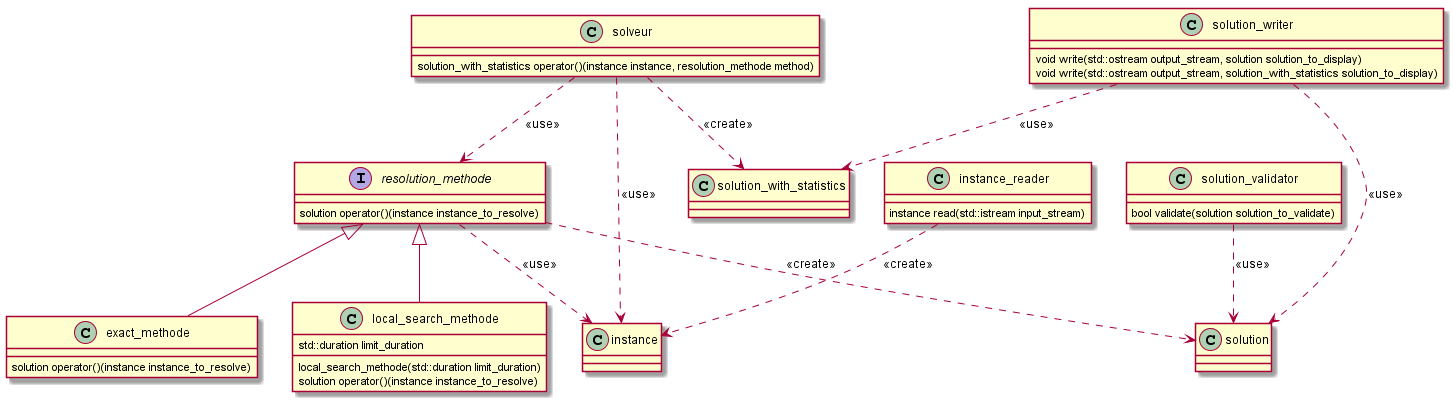
\includegraphics[width=\textwidth]{parts/analyse_et_conception/services}



%  todo : décrire les services